A variety of weak mode deformations can exist in the detector even after alignment.
As mentioned previously, these weak modes consist of misalignments which don't affect the $\chi^2$ of the residuals and thus are not handled by the basic alignment algorithm.
In the presence of a weak mode, the description of the detector geometry can still provide efficient and high quality track fits, but there may also be systematic biases in one or more track parameters.
Several weak modes, their impacts on the reconstruction, and the steps taken to eliminate them are detailed in~\cite{2014.alignment-performance-8tev, 2012.alignment-systematics}. 
This section focuses specifically on sagitta distortions that result in a bias in the reconstructed track momentum.

These \emph{sagitta} distortions consist of detector movements orthogonal to the trajectory of the outgoing particle.
The effect on the reconstructed track curvature is different for positvely and negatively charged particles, resulting in a charge-antisymmetric bias.
This effect is illustrated in the curl deformation shown in Figure~\ref{fig:align_radial_distortion}.

In the plane transverse to ATLAS's magnetic field, outgoing particle tracks form circular arcs.
The sagitta is defined as the distance from the center of this arc to the center of its base, as shown in Figure~\ref{fig:align_sagitta}, and it represents the ``amount of bending'' in the track.
In the case where the sagitta $s$ is considerably smaller than the detector radius $R_0$, which is a valid assumption when working with high momentum tracks, the transverse momentum of a particle of charge $q$ can be written as~\cite{2018.alignment-radial-distortions}:
\begin{equation}
  \pt \propto q B \frac{R_0^2}{8s}
  \label{eq:align_pt_sagitta}
\end{equation}
where $B$ is the strengh of the detector's magnetic field.
If a sagitta bias is present, the track's transverse momentum shifts by~\cite{2012.alignment-systematics}:
\begin{equation}
  q/\pt\rightarrow q/\pt+\delta_s ~~~~~\textrm{or}~~~~~ \pt\rightarrow \pt\cdot(1+q\pt\delta_s)^{-1}
  \label{eq:align_pt_sagitta_bias}
\end{equation}
where $\delta_s$ is a universal bias parameter that uniquely defines the deformation.
Finally, since the reconstructed polar angle does not change under a sagitta deformation, the longitudinal component of the momentum scales along with the transverse component, and an equivalent equation can be written for the total momentum:
\begin{equation}
  p\rightarrow p\cdot(1+q\pt\delta_s)^{-1}
  \label{eq:align_p_sagitta_bias}
\end{equation}

\begin{figure}[htbp]
  \centering
  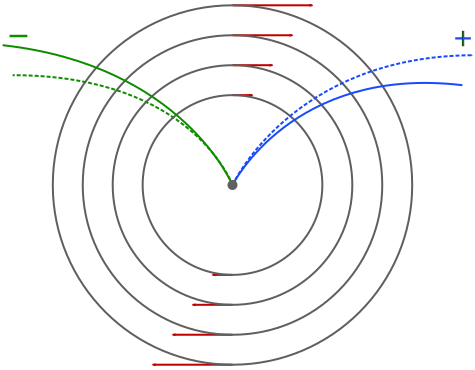
\includegraphics[width=.45\textwidth]{figs/alignment/radial-distortion}
  \caption{Representation of a curl distortion in the detector.  The image shows a cutaway in the transverse plane.  The deformation is represented by the red arrows, and the impact on the reconstructed positive (blue) and negative (green) tracks are shown.  The dashed lines represent the true particle trajectories, and the solid lines represent the reconstructed trajectories.}
  \label{fig:align_radial_distortion}
\end{figure}

\begin{figure}[htbp]
  \centering
  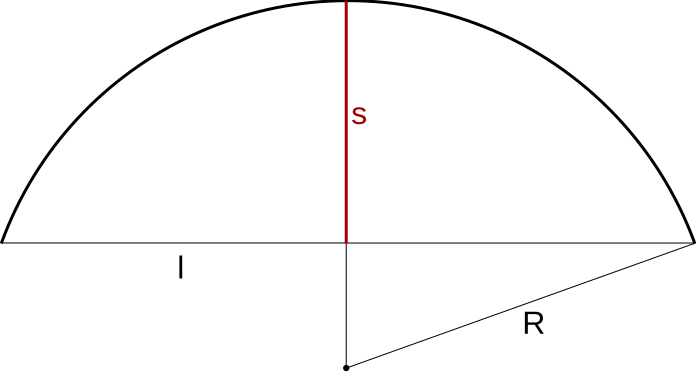
\includegraphics[width=.4\textwidth]{figs/alignment/sagitta}
  \caption{Geometric definition of the sagitta $s$ in relation to the length of the chord $l$ and the radius $r$ of a circular arc.}
  \label{fig:align_sagitta}
\end{figure}

\subsection{Sagitta bias monitoring with electron $E/p$}\label{align:eop}
Since a sagitta bias results in changes in the momentum of particles' tracks as measured by the ID, they can be identified using independent measurements from other systems in the detector.
One such method involves using the energy-momentum ratio of electrons ($E/p$).
Since the electron's energy is measured in ATLAS's calorimeter systems, it is not sensitive to any sagitta bias that may exist in the ID and the corresponding track momentum.
Under the assumption that the calorimeter response is independent of the charge of incoming particles, a charge-dependent momentum bias in the ID will manifest as a difference in the $E/p$ ratio for electrons and positrons.%\footnote{For the remainder of this section, electrons and positrons will collectively be referred to as ``electrons'' unless explicitly noted.}.

In the presence of a sagitta bias, the momentum will change according to Equation~\ref{eq:align_p_sagitta_bias} and the average measured $\eop$ can be written as:
\begin{equation}
  \eop^{\pm}\rightarrow\eop^{\pm}\pm\langle\et\rangle\delta_s
\end{equation}
where the approximation $\pt\approx\et$ is used.
Assuming that $\eop^+ = \eop^-$ in the absense of a bias, the sagitta bias parameter can be written as:
\begin{equation}
  \delta_s = \frac{\eop^+ - \eop^-}{2\langle\et\rangle}
\label{eq:align_eop_sagitta}
\end{equation}
If the kinematic selections for electrons and positrons are identical, the energy scale of the calorimeter will not factor into the $\eop$ difference; however, it will affect $\langle\et\rangle$ which would scale the measured $\delta_s$.
This is expected to be a small effect, as the energy scale for electrons has been measured at \com{13} with uncertainties on the per-mil level across the entire detector~\cite{2016.electron-photon-calibration}.

\subsubsection{Measuring $\eop$}
\TODO{selection, fit, results, recommendations alongside zmm}

\subsubsection{Results}
